% !Mode:: "TeX:UTF-8"
\chapter{模型试验以其评估}

\qquad 为了证明我们所提出模型的有效性以及合理性,我们设计了不同的实验来识别我们数据中的社交关系,并以试验结果来评估我们的模型。

\section{实验准备工作}

\subsection{数据及评估方法}

从前面的介绍中我们可以知道,我们构造的移动社交网络的数据集来自中国中部湖南省的一个县级市,具体的信息可见章节3。为了更加有效的推断用户之间的社交关系类别,我们仅仅考虑在我们网络中较为活跃的用户。这里我们定义活跃用户为在三周内至少有5个联系人与该用户进行了联系,则我们可以认为该用户为活跃用户。而我们所采集具有社交关系的用户们,他们在三周内至少进行了10次以上的通话,才可以将这些社交关系放入我们的移动社交网络当中来。需要注意一点的是,在我们的实际数据集中,并不具有朋友关系这一实际关系集合,因此我们将两个通话次数在15次以上的用户当作具有朋友关系的用户,这一方法在许多其他的研究中都得到运用\upcite{tang2012inferring}。通过这种筛选工作,构成我们移动社交网络大概有304,000活跃用户,以及两千万条稳定的社交关系。为了使得我们的结果真实可信,我们将实验重述了10次,最终展示结果取10次结果的平均值,以准确率、召唤率以及F1-Measure。这三个概念是常用来衡量机器学习分类器的指标量,具体的计算公式如下\upcite{olson2008advanced},

\begin{equation}
Precision = \frac{tp}{tp + fp} \\
\end{equation}

\begin{equation}
Recall = \frac{tp}{tp + fn} \\
\end{equation}

\begin{equation}
\bm{F1} = 2 \times \frac{Precision \times Recall}{Precision + Recall} \\
\end{equation}

其中$tp$代表实际为正的标签预测为正的总数,$tn$代表实际为正的标签预测为负的总数,$fp$代表实际为负的标签预测为正的总数,$fn$代表实际为负的标签预测为负的总数。 \\


我们核心的代码均用C++进行了实现,并且我们实现的C++代码提供了Shell接口,方便用户直接在Linux Shell命令行下进行操作。同时,我们的代码具有相当的扩展性,因为时间与篇幅的关系,我们在这里不对其进行详细赘述。除此之外,我们实验的环境都是在一个有16核,2.5G的因特尔顶级处理器,104G内存,1T SSD硬盘的谷歌服务器上进行的,充分保证了实验代码运行的速度,以及实验的稳定性。我们的代码没有采用分布式的方法,本身因为实验设备的限制,另外一个原因则是我们服务器的内存以及CPU性能相当好。因此,如果直接用并行的方法来处理实验,反而会比10台普通机器以内的分布式算法计算得更快(在消息传递时,单机传递消息在内存中传递,所耗时间非常少)。


\subsection{实验比较的方法}

我们将我们所提出的$BTFG$模型与其他的分类器算法进行对比。出了常见的分类器算法外,我们也将我们的方法与最传统的条件随机场算法进行对比。因此这些算法包括朴素贝叶斯(\textbf{Naive Bayes}),随即森林(\textbf{Random Forest}),支持向量机(\textbf{Support Vector Machine})以及条件随机场(\textbf{Conditional Random Fields})。对于朴素贝叶斯以及随机森林,我们使用\textit{Weka}\upcite{hall2009weka}来实现,并同时考虑了标签分布不平衡问题。对于支持向量机,我们采用\textit{LibSVM}\upcite{chang2011libsvm}的代码实现。对于条件随机场,我们使用所有的因子来进行训练,之后再来对测试集合来进行预测,所用工具为Mallet\upcite{McCallumMALLET}。注意到所有的比较方法我们均考虑到了标签分布不平衡问题。

对于所有的比较方法,我们全部使用了第三章所提出来的非结构特征,如时空特征等等。而对于图模型,条件随机场使用了所有的因子来构建模型,但是在训练集中进行训练,在测试集中进行测试,即测试集合训练集是两个不同的网络,并非在一个网络上进行的。而我们的$BTFG$模型,则使用了所有我们定义的因子函数来预测不同边的社交关系。这两个唯一不同的一点是,我们的方法直接在一个网络中进行推断,并没有像解决经典的分类问题一样,将数据分为训练集合测试集。因此,在训练的时候,我们可能会使用到未知的标签(将未知也看作一种类型)。


\section{实验结果}
我们在数据集上面采用不同的方法来对我们数据集中的社交关系进行预测。在预测实验中,我们使用80\%具有明确社交关系的数据,而将剩余20\%的数据看作未知的社交关系,以此作为测试。

\subsection{模型预测性能}



\begin{table}
\centering
\caption{不同分类方法在社交关系识别任务上的准确率}
\label{method-results}

\begin{tabular}{|c|c|c|c|}
	\hline
Algorithm & Prec. & Accuracy  & F1-score\\ \hline
Naive Bayes &0.663 & 0.685 & 0.673 \\ \hline
Random Forest& 0.652 & 0.703& 0.681 \\ \hline
Support Vector Machine & 0.726 & 0.720 & 0.724\\ \hline
Conditional Random Field & 0.623 & \textbf{0.903} & 0.749 \\ \hline
BTFG & 0.762 & 0.853 & \textbf{0.798} \\ \hline
\end{tabular}
\end{table}

表\ref{method-results}展示了不同分类算法在我们数据集上面的预测任务的结果。很显然,我们的$BTFG$模型比其他任何一个分类算法的效果都要好得多。而支持向量机算法是在所有非图模型算法中预测效果最好的算法。条件随机场模型比一系列的非图模型算法都要好,因为条件随机场能够已定程度刻画复杂图结构与社交关系之间的关系,而这些复杂的结构在现实生活中往往是真实存在的。我们的模型比CRF的结果更好,原因在于我们运用了完完整整的社交网络结构,而并非将数据分为训练集和测试集。将我们的模型与非图模型算法进行对比,我们的模型在准确率、召回率和F1-Measure上面比基本的分类器算法要好得多,将结果提升将近 10\%左右。除此之外,我们的基本的基础算法的识别准确率相对于其他研究来说,算是很高的结果,这也说明我们提出的时空等特征在识别不同社交关系的任务上有着较高的识别度。从识别准确率的角度来看我们的结果,总体上我们能够识别将近80\%。分别看每一类关系,我们能够识别83\%的朋友关系,70.8\%的同事关系,76.5\%的家庭关系。


\subsection{特征贡献分析}


\begin{figure}[!ht]
    \centering
    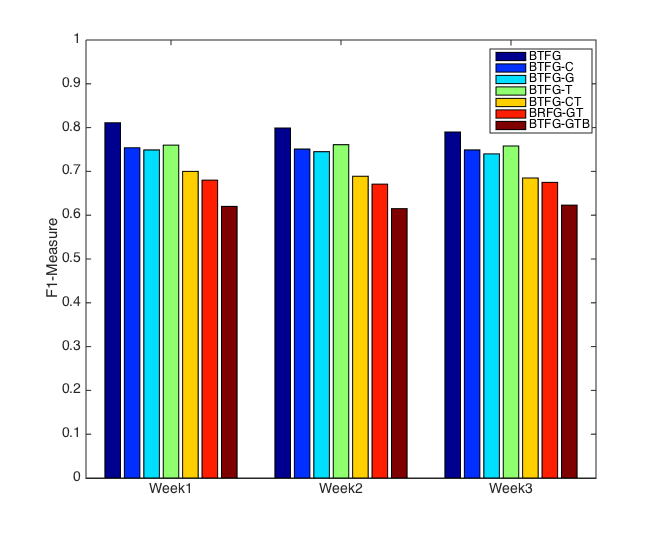
\includegraphics[scale=1, width=0.9\textwidth]{figure/fcanalysis.png}
    \caption{特征贡献分析。BTFG是提出的模型。BTFG-C是除去社交特征的模型。BTFG-G是除去时空特征的模型。BTFG-T是忽略三元结构特征的模型。BTFG-CT是同事忽略通话特征和三元结构的模型。BTFG-GT是忽略了地理特征与三元特征的模型。BTFG-BGT则是忽略了平衡因子、时空特征以及三元结构的模型。}
    \label{fig-factor-contribution-analysis}
\end{figure}


在$BTFG$模型当中,我们充分考虑了通话特征,时空特征,还有前面我们提出的因子,包括平衡因子以及三元结构因子。这里我们实验来检测这些特征对于关系识别模型的最终识别结果的影响以及贡献程度。我们首先将所有的特征放在一起进行实验,即我们所进行的原始实验。之后,我们我们一个一个按照顺序来移除这些特征,这样我们就能清楚的看清楚每一类特征对于关系识别任务预测的重要程度。特别的,我们首先一处时空特征,并将其模型成为BTFG-G,接着进一步移除三元结构特征,即BTFG-GT。最后,我们移除平衡因子记为BTFG-GTB。我们一次对每类模型进行训练任务以及预测任务。最终,我们可以在图\ref{fig-factor-contribution-analysis}中观察到,每一类特征的减少,都会带来相应的识别准确率的降低,只有当所有的因子在一起的时候识别准确率爱最高。这也充分的说明了我们的模型能够很好的将所有不同的因子函数结合起来,并且每一个因子在我们提出的方法中对于关系识别性能的预测都有提升。

\subsection{标签分布不平衡方法比较}

特别地,我们设计实验检验我们提出的解决标签分布不平衡问题方法的有效性。在表\ref{tb-imbalance-methods}中我们可以看到解决标签分布不平衡问题的各类方法的预测性能。我们在每种方法进行10次实验之后,去改方法在关系识别任务上面的平均F1 score。这也显示了在我们的模型中,使用平衡因子不仅仅能够有效改进标签分布不平衡问题,而且我们的方法比传统解决标签分布不平很问题的方法进行比较的时候,我们的方法用来进行关系识别任务要好得多,这也证明了我们所提出的想法的正确性。而使用下采样的结果远比另外两种方法要差,我们认为造成这一现象的原因是由于下采样之后,整个网络中的数据量较少,破坏了原始的网络结构,删去了一些非常重要的点和社交关系边,而剩余的节点与边并不能很有效的帮助模型来进行关系识别任务。


\begin{table}
\center
\caption{各种解决标签分布不平衡问题的F1-Measure Score}
\label{tb-imbalance-methods}
\begin{tabular}{|c|c|c|c|}
\hline
Methods & Families & Colleagues & Friends \\ \hline \hline
BTFG-B &0.781 & 0.743 & 0.92 \\ 
Undersampling & 0.701 & 0.642 &0.803 \\ 
Oversampling & 0.787 & 0.741 & 0.89\\ \hline
\textbf{BFTG} & \textbf{0.798} &  \textbf{0.754} & \textbf{0.92} \\ \hline
\end{tabular}
\end{table}


\subsection{标签不平衡比例实验}
我们进一步的测试了我们提出平衡因子方法的鲁棒性。图\ref{fig-imbalance-ratio}显示了在不同关系比例的数据集上关系识别任务的F1 Score。为了使得实验更加简单有效,我们让两种关系的比例保持一致的同时,再调整剩余的标签数据的比例。结果可以看到,在不同的情形下我们的结果稳定性相当好,最差的情形仅仅损失了大约2\%的F1 Score。



\begin{figure}[ht]
    \centering
    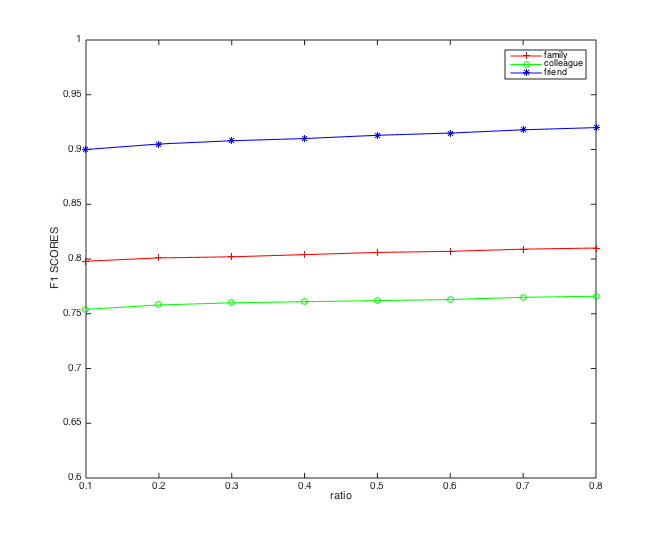
\includegraphics[scale=1, width=0.9\textwidth]{figure/RatioPer.png}
    \caption{不同比例的不平衡数据集实验结果}
    \label{fig-imbalance-ratio}
\end{figure}


















































